\documentclass[11pt, a4paper]{article} 

% Packages
\usepackage[fleqn]{amsmath} % fleqn: flush left equations <-- Left-flush equations
\usepackage{graphicx}

% Format
\usepackage[margin=2cm, top=2cm]{geometry}

% Heading
\title{\bf Design 1\\[1ex]
\rm\normalsize CS202 Programming Systems, Summer 2020 }
\date{\normalsize Due: July, 2, 2020}
\author{\normalsize Armant Touche}

\begin{document}

\vspace{0cm}\maketitle 

\section*{UML Diagram:}


            \begin{center}
            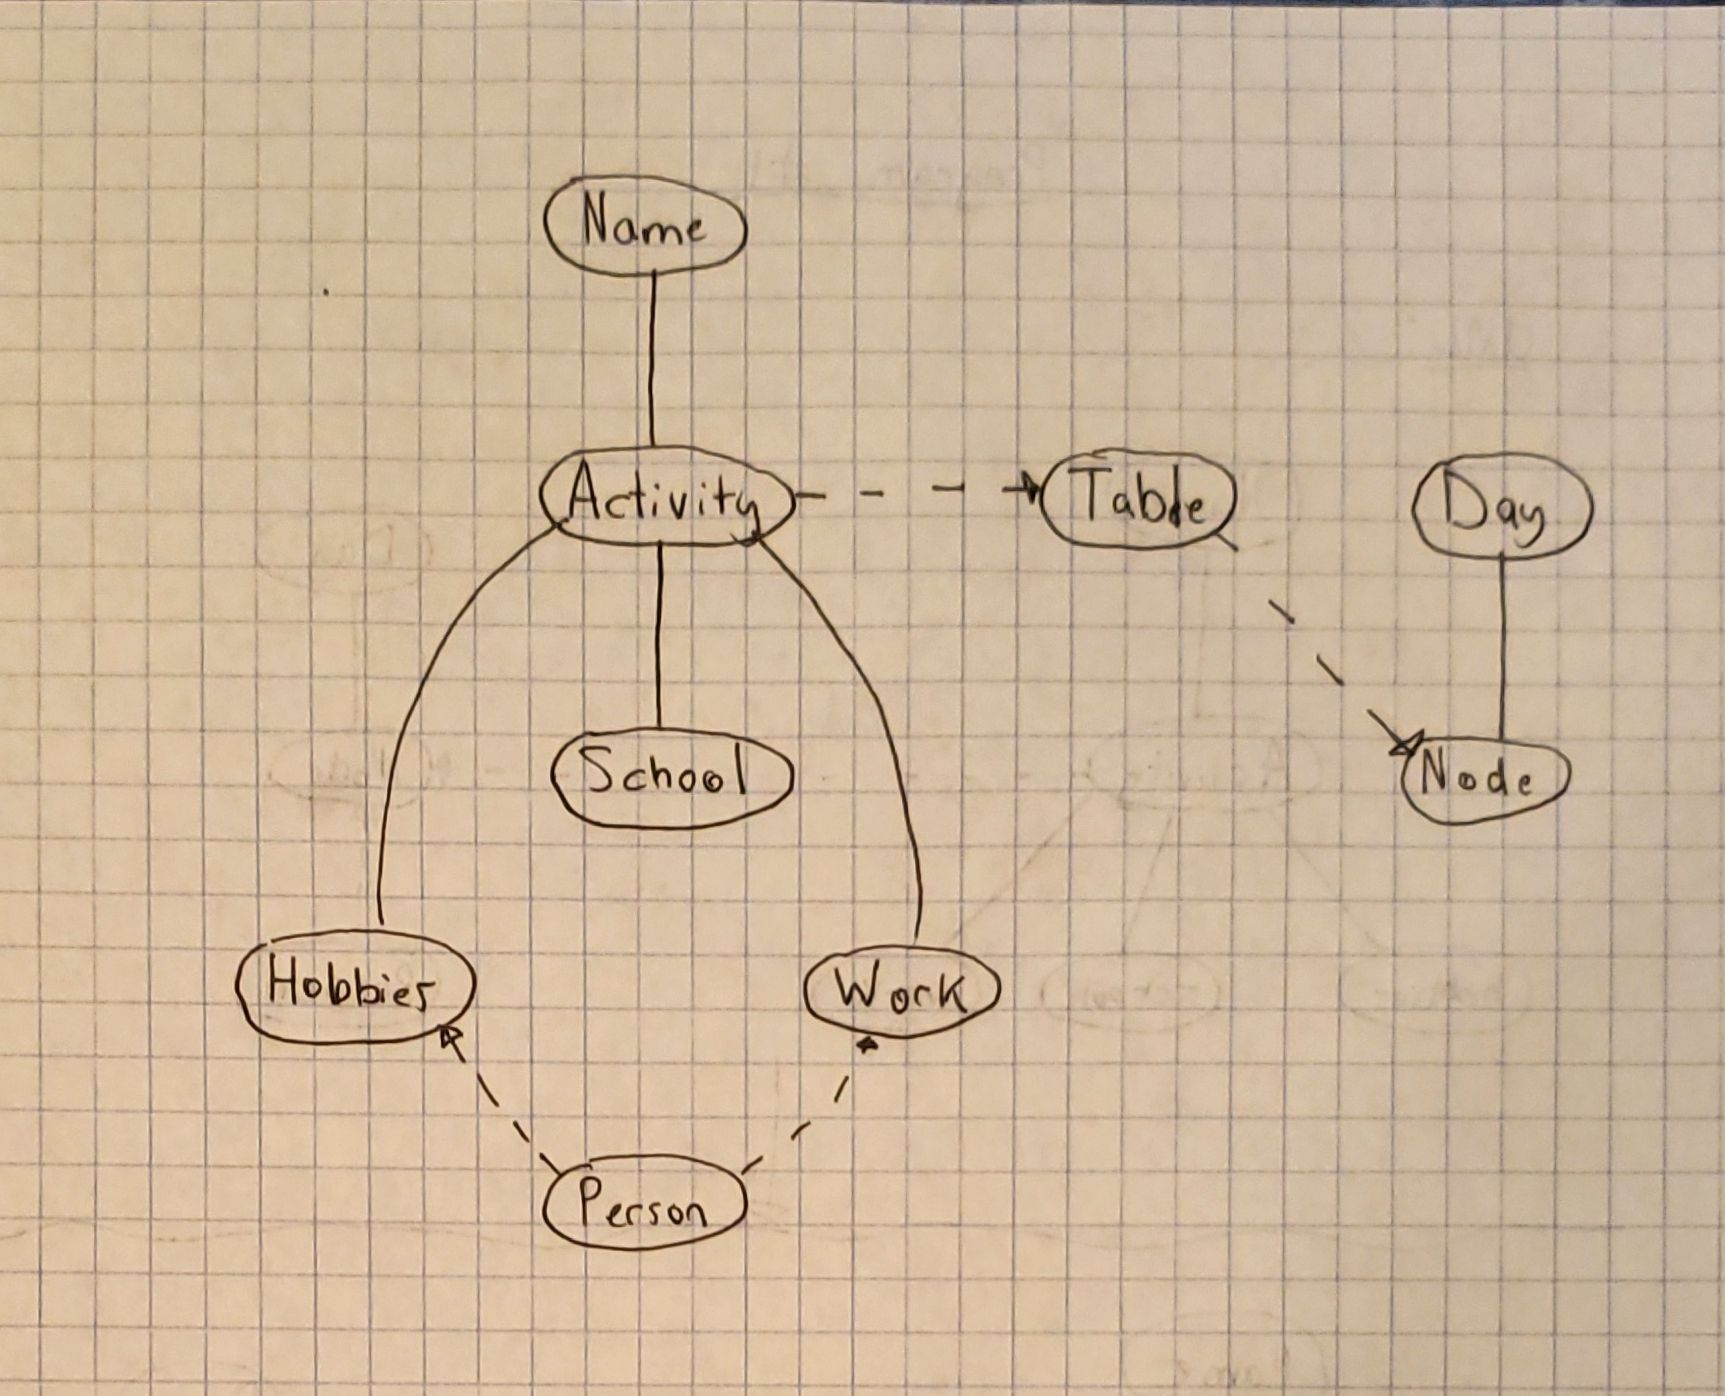
\includegraphics[width=.5\textwidth]{uml1}
            \end{center}

\section*{Write-up:}

This program will be a time managements application that will keep track of "activities." For my base class in the single-inheritance hierarchy, name will be the parent. Then activity will be the subclass of name. To fulfill the three distinct activity requirement, I will have three classes that are derived from activity which will be: (i) hobbies (ii) school (iii) work. To management activity's data, I will have  an array of doubly linked list of node-type which will be "contained" in the activity class since we are cataloging. The node class will be derived from day class so I can keep track of which days have any certain types of activity. To create interacting relationship between the three activity classes, I will have person class that will contain the node class which will person to interact with activity and it's derived classes: (i) hobbies (ii) school (iii) work. The derived class, work, will support the "at least 6 hours every day and at most 8 hours" requirement because work should last between 6 hours and 8 hours because going to school and hobbies are time demanding. For the name, I will have three constructors where the first one set the data members to their zero equivalency, second constructor will intake a character pointer called name of activity, and the third constructor will intake itself as a copy constructor. For the public section of name, I will have: (i) read in function for name of activity (ii) display name (iii) copy name function (iv) remove activity. In the protected section: (i) character pointer for name. Derived from name, activity class which will following the convetion of having a default constructor, copy constructor, and a constructor that will intake a character pointer for category of activity. For the derived activity class, in the public section: (i) function for reading in category of activity (ii) function to display activity (iii) function to copy activity. In activity's protected section: (i) character pointer for category of activity (ii) integer value for length of activity in hours (iii) table pointer to my array of nodes which will contain the days of the week. Then I will have three classes that derive from activity: (i) hobby (ii) school (iii) work. For hobby class I will have: (i) wrapper function to display from activity.  For work class I will have: (i) wrapper function to display from activity. For school class I will have: (i) wrapper function to display from activity. Then I will have a person class that will contain: (i) hobby (ii) work (iii) school. For table, in the public section: (i) wrapper function to create a node (ii) function to traverse table (iii) function to hash (iv) function to check if table exists (v) function to search. For table, in the private: (i) node double pointer (ii) recursive function to traverse (iii) recursive function to search. For node, in the public section: (i) traverse doubly linked list (ii) function to search doubly linked list (iii) remove from doubly linked list. In the private section: (i) recursively traverse doubly linked list (ii) recursively search doubly linked list (iv) node pointer called next. Node protected section: (i) have day as member. Node will be derived from day since we are keeping tracked of which days has activities. For may day class, in the public section: (i) read in the name of day function (ii) display name of day. For day, in the protected section: (i) character pointer for name of day. For all of my classes, destructor for all my classes. My client program create an activity object and depending on the user choice, I pass the object to the three derived classes to be copied and the activity class, will pass an integer value to table for hashing, based off the choice of day.

\end{document}
